\documentclass[10pt,a4paper]{article}
\usepackage[utf8]{inputenc}
\usepackage[italian]{babel}
\usepackage{amsmath}
\usepackage{amsfonts}
\usepackage{amssymb}
\usepackage{graphicx}
\usepackage{gensymb}
\usepackage[left=2cm,right=2cm,top=2cm,bottom=2cm]{geometry}
\newcommand{\rem}[1]{[\emph{#1}]}

\author{Gruppo BN \\Lisa Bedini,  Federico Belliardo, Marco Costa}
\title{Esperienza 12: Flip-Flop e contatori}

\begin{document}
\maketitle

%TODO - Secondo me in tutta la relazione le immagini non sono il massimo avrei voluto mettere le immagini del flip-flop congelato, ma non le abbiamo prese. Le immagini che mostrano le misure dei tempi non sono il massimo. Io le toglierei.

\section{Scopo dell'esperienza}
Lo scopo dell'esperienza è di montare e verificare il corretto funzionamento di 4 circuiti: Flip-Flop D-Latch, divisore di frequenza, shift register e generatore di sequenze pseudo-casuali.

\section{Materiale a disposizione}
\begin{itemize}
\item SN74LS00 Quad NAND gate
\item SN74LS94 4-bit binary counter
\item SN74LS74 Dual D-Latch
\item SN74LS86 Quad XOR gate
\item DIP switch
\item 4 LED
\end{itemize}
I valori delle componenti sono state misurate con multimetro digitale (incertezza riportata sul manuale).
Le differenze di potenziale sono state misurate tramite oscilloscopio, se non indicato diversamente, e come incertezza si è presa la sensibilità dei cursori più il 3\% di calibrazione.
Per misurare i tempi si è usato l'oscilloscopio e come relativa incertezza si è preso il massimo fra la sensibilità dei cursori e la semidispersione dei valori plausibili.

\section{Flip-Flop D-Latch}
%Sono perplesso dalle prime tre figure... In particoalre dalla prima
Si è realizzato un circuito Flip-Flop di tipo D-Latch, come mostrato in figura \ref{circuito}, utilizzando le porte NAND di due integrati. L'ingresso D, che corrisponde al dato da memorizzare, è stato collegato all'impulsatore realizzato con Arduino Nano. L'Enable è collegato alla terra attraverso uno switch manuale. La tensione di lavoro durante tutta l'esperienza è stata fissata a: $V_{CC} = 4.85 \pm 0.03$V (misurata tramite multimetro digitale, con incertezza presa dal manuale).\\ 

\begin{figure}[!htb]
\centering
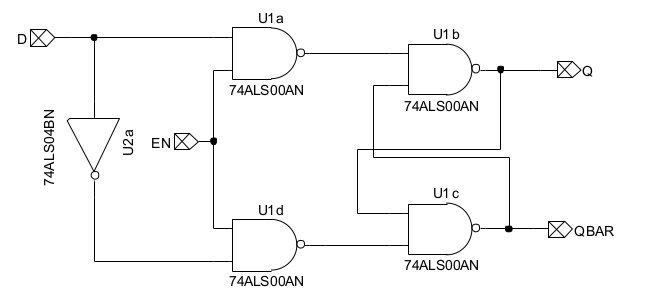
\includegraphics[scale=0.7]{flipflopDlatch.png}
\caption{Circuito D-Latch NAND.\label{circuito}}
\end{figure}

In figura \ref{segue} si vede come il segnale $Q(t)$ in uscita dal Flip-Flop segua l'ingresso quando enable è alto riproducendo la tabella \ref{stati2}.\\

\begin{figure}[!htb]
\centering
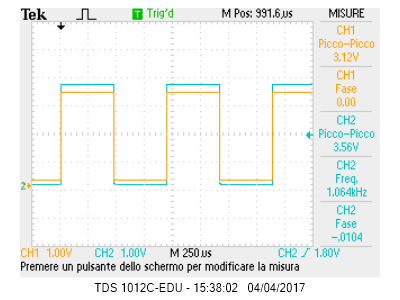
\includegraphics[scale=1.0]{FFD1in2Q.png}
\caption{Segnali D e Q quando enable è alto.\label{segue}}
\end{figure}

\begin{table}[!htb]
\centering
\begin{tabular}{|c|c|c|c|c|}
\hline 
EN & D & S & R & Q\\ 
\hline 
1 & 1 & 0 & 1 & 1\\ 
\hline 
1 & 0 & 1 & 0 & 0\\ 
\hline 
0 & 1 & 1 & 1 & Hold\\ 
\hline 
0 & 0 & 1 & 1 & Hold\\ 
\hline 
\end{tabular}
\caption{Tabella degli stati per un Flip-Flop NAND. \label{stati2}}
\end{table}

Commutando manualmente lo switch e impostando dunque $EN = 0$ il Flip-Flop rimane congelato nello stato in cui si trovava prima della commutazione.
Affinchè il valore che il Flip-Flop memorizza sia deterministico è necessario che la commutazione dello switch non avvenga durante gli hold-time e setup-time del Latch. Quando il bit di enable è disattivato entrambe le uscite dei NAND del primo livello sono a 1 pertanto il Latch è nello stato di hold.\\

Essendo il Latch costruito con delle porte NAND ho una situazione di instabilità quando gli ingressi delle porte sul secondo livello sono entrambe a 0. Questo può succedere solo se gli ingressi di tutte le porte sul primo livello sono 1. Il NOT tra i due ingressi evita questa situazione.\\
L'enable è attivo alto. Cioè quando $enable = 0$ ho permanenza dello stato, infatti gli ingressi al secondo livello dei NAND sono sicuramente a 1, mentre posso avere evoluzione dello stato se il bit $enable = 1$.\\
Quando l'ingresso enable è lasciato flottante il NAND forza la tensione a $5$V quindi il valore logico è   $enable = 1$ e l'uscita insegue l'ingresso, lo switch collega l'enable alla tensione di terra, dunque se chiudo l'interruttore l'enable viene forzato al valore logico basso e il Flip-Flop entra nello stato \emph{hold}.%si capisce male cosa vuoi dire: lo stato di hold sbaglio o lo hai descritto subito sopra?\\ A me sembrano spiegazioni complementari.

Si sono misurati i tempi di ritardo sulla salita e discesa delle uscite del Flip-Flop rispetto all'ingresso (uscita del pulsatore). I tempi sono stati presi misurando la differenza di tempo fra i punti $t_{HL}$ per le discese oppure $t_{LH}$ per le salite dei due segnali con potenziale pari a metà delle rispettive $V_{PP}$\footnote{Per le misure ci siamo aiutati con i cursori che ci mostravano contemporanemante le coordinate temporali e il potenziale. Come incertezza si è presa la semidispersione dei tempi di ritardo in corrispondenza dei punti che avevano il potenziale richiesto entro l'errore dei cursori}. Le misure sono riportate nella tabella \ref{ritardo} sia per l'uscita $Q$ che per l'uscita $\bar{Q}$.

\begin{table}[!htb]
\centering
\begin{tabular}{|c|c|c|}
\hline 
• & $t_{LH}$ (ns) & $t_{HL}$ (ns)\\
\hline
$Q$ & $36 \pm 2$ & $34 \pm 4$\\
\hline
$\bar{Q}$ & $36 \pm 2$ & $36 \pm 2$\\
\hline
\end{tabular}
\caption{Misure dei tempi di ritardo in salita e discesa per il Flip-Flop.\label{ritardo}}
\end{table}

Tutti e quattro i tempi sono risultati compatibili tra di loro.\\
%Il tempo tipico di commutazione di una porta NAND è tra i $9$ns e i $15$ns. I valori %misurati di circa $36$ns sono perfettamente compatibili con il tempo di commutazione di 4 %porte NAND ($9 \cdot 4 = 36$ns).\\
%non cpaisco bene perchè siano 4 commutazioni in serie: direi 2 più al max una per il not, ma non capisco perchè, sebbene ci siano 4 not, le commutazioni debbano avvenire una dopo l'altra e non a coppie di due.\\ Infatti dovrebbe essere come dici tu ma se è vero allora non mi sembra compatibile quel tempo cn quello di commutazione di due porte e toglierei questa spiegazione.

Di seguito sono riportate le immagini delle misure dei tempi di ritardo sull'oscilloscopio per l'uscita $Q$ solamente:\\

\begin{figure}[!htb]
\centering
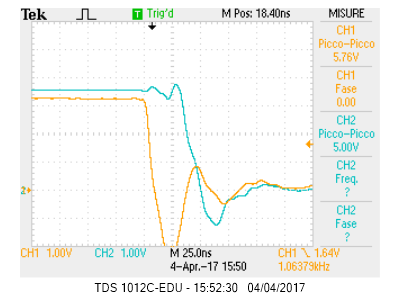
\includegraphics[scale=1.0]{tphlQ.png}
\caption{Tempo di ritardo  $t_{HL}$ rispetto a D (CH1) per l'uscita $Q$ (CH2).\label{q1}}
\end{figure}

\begin{figure}[!htb]
\centering
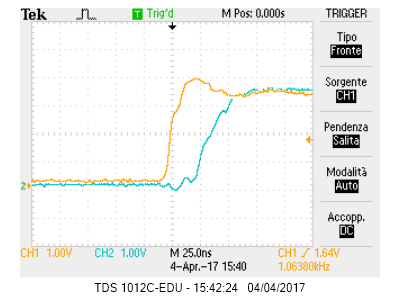
\includegraphics[scale=1.0]{tplhQ.png}
\caption{Tempo $t_{LH}$ per l'uscita $Q$ (CH2).\label{q2}}
\end{figure}


\section{Divisori di frequenza}
Si è realizzato un contatore a 4 bit come in figura \ref{contatore} connettendo l'uscita Q del primo JK (FF1) al clock del secondo JK (FF2),i restanti JK sono già interconnessi all'interno del package. Si vogliono utilizzare tutti i JK in modalità Toggle, cioè in modo che oscillino tra lo stato 0 e 1 alla transizione basso-alto del clock (per costruzione). Per fare ciò è necessario che l'ingresso J di ogni Flip-Flop sia impostato a 1; questa configurazione è realizzata ponendo $R_0$ a terra e $R_1$ flottante (per il momento).\\
Infatti la configurazione toggle del JK si ottiene se $J = 1$ e $K = 1$. Se K è flottante questo assume sempre il valore logico 1, e se uno degli ingressi del NAND ($R_0$ nel nostro caso) è forzato a 0 la sua uscita sarà sempre 1. Con questa scelta quindi si soddisfano le condizioni richieste per i JK.\\  
Poiché la transizione del valore di uscita Q di ognuno degli FF avviene con una frequenza dimezzata rispetto a quella del clock, le varie uscite $Q_i(t)$ oscillano con frequenze $\frac{1}{2}, \frac{1}{4}, \frac{1}{8}, \frac{1}{16}$ della frequenza di CLK1 in quanto l'uscita $Q_i$ di un FF è il clock del successivo.\\
Ogni uscita $Q_i$ è stata collegata a terra attraverso un LED e una resistenza (per limitare la corrente sul LED). Questo e l'accorgimento di impostare un clock per il FF1 di circa 1 Hz (generato con il generatore di funzioni)%mi pareva fosse il generatore di funzioni ma non dovrebbe cambiare il succo
 rende osservabili ad occhio le transizioni.\\
Interpretando il bit più a sinistra come bit meno significativo (1 per LED acceso e 0 per LED spento) si ottiene la rappresentazione fisica dei numeri da 0 a 15 in binario.\\

\begin{figure}
\centering
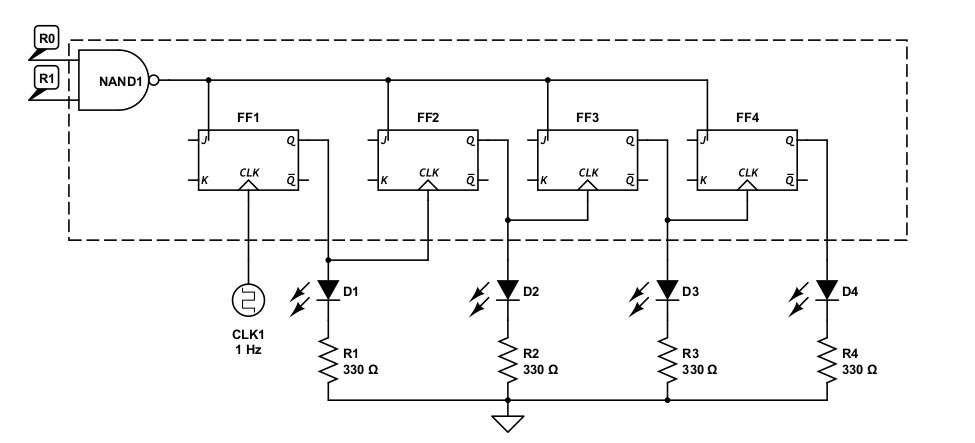
\includegraphics[scale=0.5]{divisore.png}
\caption{Contatore a 4 bit.\label{contatore}}
\end{figure}

Si è inviato in ingresso un segnale di frequenza $f_0 = 61 \pm 1$kHz e periodo $T = 16.40 \pm 0.02 \mu s$, si sono misurate le frequenze dei segnali $Q_i$ e i tempi di ritardo per la salita e la discesa rispetto al clock, definiti come differenza temporale tra i punti in cui i due segnali raggiungono la metà del rispettivo valore massimo quando avvengono le transizioni.\footnote{La misura è stata eseguita nello stesso modo dei tempi di ritardo della sezione precedente}\\

Nelle figure successive si riportano le uscite $Q_A$, $Q_B$, $Q_C$, $Q_D$ visualizzate insieme al clock in ingresso. Si può osservare dal frequenzimetro dell'oscilloscopio come le frequenze rispettano la serie geometrica descritta precedentemente.\\

\begin{figure}
\centering
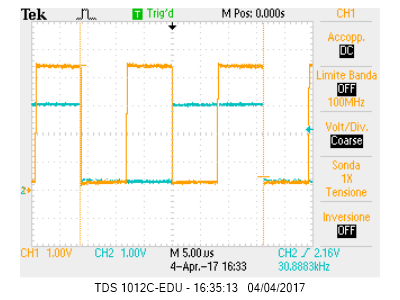
\includegraphics[scale=1.0]{QA1-2.png}
\caption{Segnale all'uscita $Q_A$ con frequenza $f_0/2$.\label{freq2}}
\end{figure}

\begin{figure}
\centering
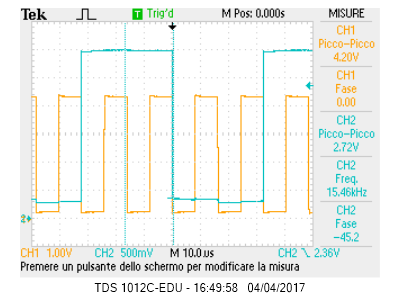
\includegraphics[scale=1.0]{QB1-4.png}
\caption{Segnale all'uscita $Q_B$ con frequenza $f_0/4$.\label{freq4}}
\end{figure}

\begin{figure}
\centering
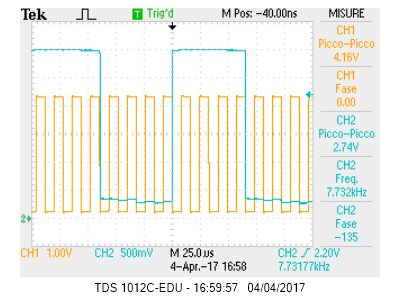
\includegraphics[scale=1.0]{QC1-8.png}
\caption{Segnale all'uscita $Q_C$ con frequenza $f_0/8$.\label{freq8}}
\end{figure}

\begin{figure}
\centering
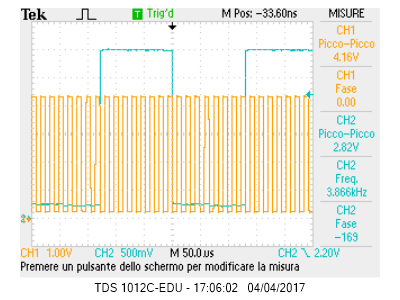
\includegraphics[scale=1.0]{QD1-16.png}
\caption{Segnale all'uscita $Q_D$ con frequenza $f_0/16$.\label{freq16}}
\end{figure}

%Il tempo di ritardo è definito come l'intervallo temporale tra i punti in cui i due segnali raggiungono le rispettive metà. ripetizione\\

\begin{table}[!htb]
\centering
\begin{tabular}{|c|c|c|c|c|}
\hline 
• & $T (\mu \mbox{s})$ & $f (mbox{kHz})$ & $t_{HL}$ (ns) & $t_{LH}$(ns) \\ 
\hline 
$Q_A$ & $32.4 \pm 0.03$ & $30.8 \pm 0.3$ & $44 \pm 2$ & $43 \pm 2$ \\ 
\hline 
$Q_B$ & $65.2 \pm 0.7$ & $15.3 \pm 0.2$ & $55 \pm 2$ & $54 \pm 2$ \\ 
\hline 
$Q_C$ & $129 \pm 1$ & $7.75 \pm 0.07$ & $69 \pm 2$ & $66 \pm 2$ \\ 
\hline 
$Q_D$ & $258 \pm 2$ & $3.88 \pm 0.03$ & $83 \pm 2$ & $79 \pm 2$ \\ 
\hline 
\end{tabular} 
\caption{Misure di frequenza e tempi di propagazione per il divisore. \label{misureDivisore}}
\end{table}

Di seguito sono riportate le immagini relative alle prese dei tempi di ritardo di $A$ a scopo esemplificativo:

\begin{figure}
\centering
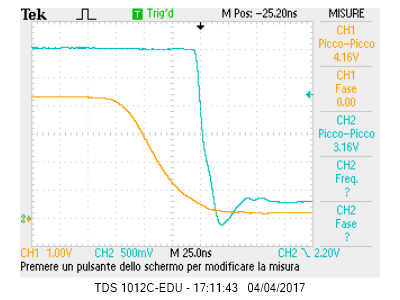
\includegraphics[scale=1.0]{tphlQA.png}
\caption{Misura del tempo $t_{HL}$ per l'uscita $Q_A$.\label{qa1}}
\end{figure}

\begin{figure}
\centering
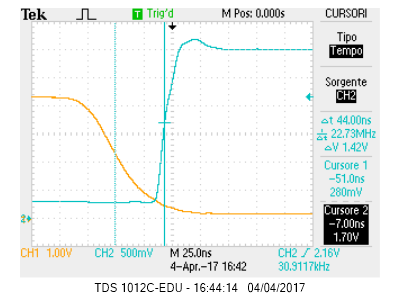
\includegraphics[scale=1.0]{tplhQA.png}
\caption{Misura del tempo $t_{LH}$ per l'uscita $Q_A$.\label{qa2}}
\end{figure}


I tempi di ritardo misurati sono tempi di propagazione attraverso la rete dei Flip-Flop e dalle misure eseguite aumentano linearmente con il numero di porte del circuito. Gli errori sui tempi $t_{HL}$ e $t_{LH}$ sono dello stesso ordine di grandezza della differenza tra essi. Questo non ci permette di eseguire considerazioni significative sul parametro $t_{HL}$ - $t_{LH}$.\\

Si vuole realizzare un contatore decadico sincrono, cioè attivare il reset quando il contatore raggiunge il valore 10. Per identificare il valore 10 sulle uscite $Q_i$ si esegue un NAND tra le uscite $Q_2$ e $Q_4$, che da un segnale basso non appena i due bit sono attivati per la prima volta (cioè si raggiunge il 10). \\
Il reset dei JK si ottiene per $J = 0$ e $K = 1$, dunque K viene sempre lasciato flottante.\\
A questo punto sarebbe possibile fornire questo valore agli ingressi di reset del circuito, tuttavia per costruire un reset sincrono con il clock si utilizza un D-Latch al cui ingresso è collegata l'uscita del NAND.\\
Il bit di reset $R_0$ viene collagato a 1 attraverso una resistenza, il bit $R_1$ è collegato all'uscita negata del Latch in modalità enabled. In questo modo l'uscita $\bar{Q}$ diventa 1 non appena si raggiunge 10 sincronamente con il clock.
%Era una frase inutile
Se non è ancora stato raggiunto il 10 vale $Q = 1$, $\bar{Q} = 0$ e dunque tutti i FF sono in modalità toggle (J = 0, NAND 1 = 1, K = 1) e il conteggio continua. Non appena $\bar{Q} = 1$ , cioè ho raggiunto il 10, l'uscita degli FF viene impostata a 0, infatti J = 1, NAND 1 = 0, K = 1, che sappiamo corrispondere al settaggio di $Q = 0$.\\
Si verifica che collegando il D-Latch allo stesso clock del contatore alla fine del ciclo i quattro LED visualizzano per mezzo ciclo di clock il valore 10 e poi passano a visualizzare lo 0. Questo problema si può risolvere collegando il D-Latch al clock negato. Con questo accorgimento il numero 9 permane per il tempo corretto (come si può verificare all'oscilloscopio) per poi passare allo zero.\\


\begin{figure}[!htb]
\centering
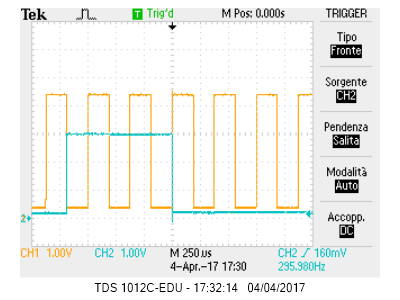
\includegraphics[scale=1.0]{clocksbagliato.png}
\caption{Segnale $Q_D$ e clock nel caso in cui FF e contatore abbiano stesso clock.\label{sbagliato}}
\end{figure}

\begin{figure}[!htb]
\centering
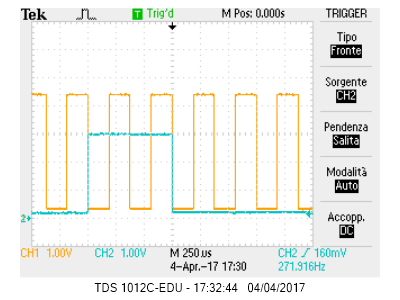
\includegraphics[scale=1.0]{clockgiusto.png}
\caption{Segnale $Q_D$ e clock nel caso in cui FF e contatore abbiano clock invertiti.\label{giusto}}
\end{figure}

Le due figure \ref{sbagliato} e \ref{giusto} mostrano l'uscita $Q_D$ nel caso di collegamento sbagliato o giusto del clock (secondo quanto detto precedentemente). Si può vedere che \ref{sbagliato} mostra come $Q_D$ rimanga acceso per mezzo ciclo di clock più del dovuto questo causa il comportamento indesiderato descritto precedentemente.\\
Ciò è dovuto al fatto che il contatore e il Flip-Flop sono sensibili rispettivamente al fronte di discesa e di salita del clock.\\

\section{Shift register con D-Latch}
Abbiamo montato lo shift register come indicato in figura \ref{shift}. Si possono osservare gli stati dei vari Flip-Flop attraverso i diodi LED. Si è verificato che il pulsante di preset imposta tutte le uscite di Q al valore alto. Quando si collega l'ingresso D a terra chiudendo lo switch si vedono i LED spegnersi in sequenza sincronamente con il clock come atteso. Si è visto che per fare funzionare correttamente il circuito abbiamo avuto bisogno di inserire resistenze di pull-up di circa $1.5 \mbox{k}\Omega$, in particolare ai clear per tenerli al valore alto. Una maggior stabilità del sistema si poteva ottenere anche collegando il preset al valore alto della tensione attraverso una resistenza durante il funzionamento del circuito.

\begin{figure}
\centering
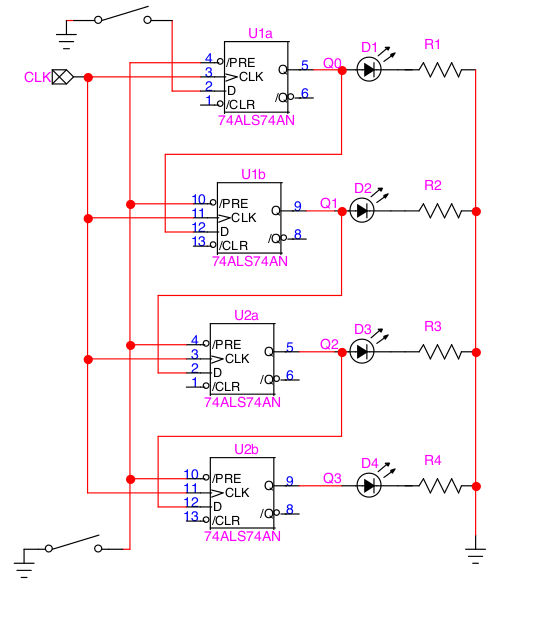
\includegraphics[scale=0.5]{shift.png}
\caption{Shift register.\label{shift}}
\end{figure}

\section{Generatore di numeri casuali}
Si è realizzato il circuito in figura \ref{pseudo} e inviando un clock a bassa frequenza si è osservata (e riportata in tabella \ref{CD}) la sequenza generata, che come si vede è completa. 
Lo XOR è stato posto tra le uscite C e D e il risultato è stato mandato in input al primo  D-Latch.\\

\begin{table}[!htb]
\centering
\begin{tabular}{|c|c|}
\hline 
1111 & 15 \\ 
\hline 
1011 & 11 \\ 
\hline 
0011 & 3 \\ 
\hline 
0010 & 2 \\ 
\hline 
0100 & 4 \\ 
\hline 
1000 & 8 \\ 
\hline 
0001 & 1 \\ 
\hline 
0110 & 6 \\ 
\hline 
1100 & 12 \\ 
\hline 
1001 & 9 \\ 
\hline 
0111 & 7 \\ 
\hline 
1010 & 10 \\ 
\hline 
0101 & 5 \\ 
\hline 
1110 & 14 \\ 
\hline 
1101 & 13 \\ 
\hline 
\end{tabular}
\caption{Tabella di numeri generata da XOR tra $Q_C$ e $Q_D$.\label{CD}} 
\end{table}

\begin{figure}[!htb]
\centering
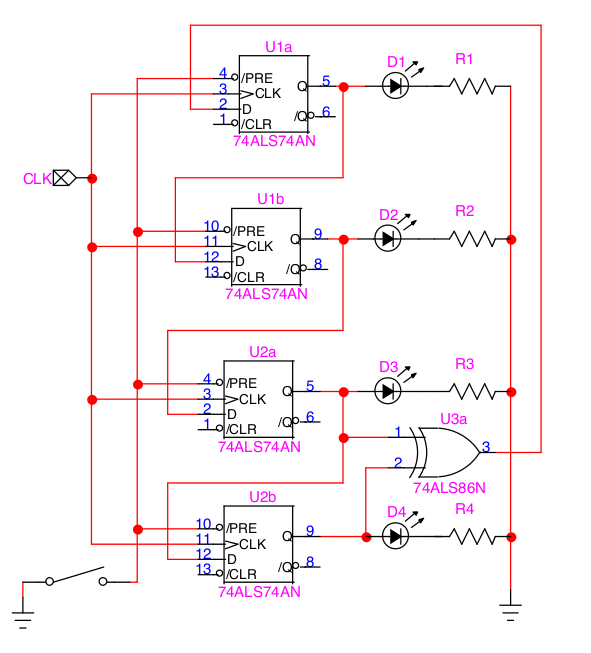
\includegraphics[scale=0.5]{pseudi.png}
\caption{Generatore di numeri pseudo-casuali.\label{pseudo}}
\end{figure}

Si è provato ad inserire lo XOR anche tra le uscite $Q_A$ e $Q_D$ del contatore per poi rimandare l'uscita di questo all'ingresso del primo D-Latch. Il risultato è riportato di seguito e non è una sequenza completa.

\begin{table}[!htb]
\centering
\begin{tabular}{|c|c|}
\hline 
1111 & 15 \\ 
\hline 
1011 & 11 \\ 
\hline 
0111 & 7 \\ 
\hline 
1010 & 10 \\ 
\hline 
0001 & 1 \\ 
\hline 
0110 & 6 \\ 
\hline 
1100 & 12 \\ 
\hline 
1101 & 13 \\ 
\hline 
\end{tabular}
\caption{Tabella di numeri generata da XOR tra $Q_A$ e $Q_D$.\label{AD}}  
\end{table}

%Manca discussione teorica su quali altri tap dsi potevano utilizzare. Galois/Fibonacci  ecc... E non intenzione di farla.
\section{Conclusioni}
Il comportamento dei circuiti montati è in accordo con quanto atteso. Per il corretto funzionamento dello shift register e del generatore di sequenze pseudo-casuali è stato necessario utilizzare resistenza di pull-up per collegare ad a $V_{CC}$ i clear.
Per il generatore di sequenze abbiamo provato ad utilizzare lo XOR anche in altre configurazioni, ma non si sono ottenute sequenze complete.
\end{document}







